% !TeX document-id = {b0ca628d-fa0a-486c-ae9b-26ef260b81e9}
%!TEX TS-program = pdflatex
%!GEDIT texbin = /usr/local/texlive/current/bin/x86_64-linux/pdflatex
% Local IspellDict: en
%
% Documentation for the DBIS Group style LaTeX template
%
% Copyright © 2013-2020 DBIS Group, WWU Münster, in particular:
%   Till Haselmann <haselmann@wi.uni-muenster.de>
%   Jens Lechtenbörger <lechten@wi.uni-muenster.de>
%   Florian Stahl  <flst@wi.uni-muenster.de>
% All rights reserved.
%


% documentation.tex
%
% Basic file to demonstrate the usage of the DBIS Group LaTeX template.
% You can build your own paper/thesis on top of this file.  Simply adjust
% all metadata and delete the inclusion of documentation-preamble
% Then, change the inclusion of documentation-body to your own file.
%

\documentclass[
%    dbisthesis=false,        % Set to false for jointly supervised thesis.
%    license=cc-by-sa,        % Publish under free and open license.
    disabletodonotes,         % Do not show todo notes in final PDF.
    language=german           % Set language: "english" or "german"
  ]{dbisseminar}
\ifthenelse{\boolean{dbispaper@dbisthesis}}{}{%
  \renewcommand{\cProf}{Prof. Dr. Heike Trautmann\\Prof. Dr. Gottfried Vossen}}

% Author(s) of paper
% Format like this: Firstname Lastname \email{Email Address}
% Multiple authors can be separated by "\and".
% (In case of multiple authors, no consent form for plagiarism checks
% is produced.  In that case, please use forms provided over there and
% hand them in separately:
% http://www.wiwi.uni-muenster.de/pruefungsamt/downloads/downloads.html)
\author{%
  Kira Alberding \email{k{\_}albe09@uni-muenster.de} % \and
  %Till Haselmann \email{haselmann@wi.uni-muenster.de}
}

% Topic of paper
\title{Entwicklung einer webbasierten kollaborativen Karteikarten-Software nach Anforderungen von OER}

% Due date of paper in format YYYY-MM-DD
\date{2021-01-18}

% Responsible supervisor(s) at DBIS Group
% Multiple supervisors can be separated by \and
\supervisor{Dr.\ Jens Lechtenbörger}

% Title of seminar
\seminartitle{Open Education Resources}

% Place and date of handing in the paper (for plagiarism declaration)
% For the date field use the following convention:
%   German date   -> dd.mm.yyyy       e.g.: 31.05.2011
%   English date  -> Month dd, yyyy   e.g.: May 31, 2011
\placeOfSignature{M{\"u}nster}
\dateOfSignature{18 Januar 2021}
\studentNumber{417911}
\studentAddress{Rudolf-Harbig Weg 46, 48149 M{\"u}nster}
\courseOfStudy{Wirtschaftsinformatik} % or Information Systems

\include{documentation-preamble}

\begin{document}
  % Create title page
  \maketitle

  \frontmatter


  %Abstract
  \begin{abstract}
Karteikarten sind eine der beliebtesten Lernmethoden, nicht nur für Schüler und Studenten, sondern auch für viele weitere Anspruchsgruppen. Zu den Inhalten zählen schon längst nicht mehr nur Sprachvokabeln, die eher eine geringere Funktionalität erfordern. Auch andere Fachbereiche finden hier Einzug, wie beispielsweise Mathematik und Chemie, die allerdings erweiterte Funktionen, wie die Eingabe von Formeln verlangen. Diese sind jedoch nach Durchführung der noch folgenden Evaluation nicht sehr häufig in denen am Markt befindlichen Anwendungen vorhanden. Ein weiteres Defizit der Angebote besteht in der fehlenden Möglichkeit zur Zusammenarbeit mit anderen Lernenden. Zwar lassen sich oft Kurse bzw. Kollektionen teilen, jedoch fehlt der gemeinschaftliche Zugriff in Echtzeit oder die Bewertungsmöglichkeiten für einzelne Karteikarten, um geringwertige Karten auszusortieren. Mit Berücksichtigung der Anforderungen des Prinzips Open Educational Resources (OER) wird im Rahmen dieser Seminararbeit eine webbasierte Anwendung entwickelt, die den Bildungszugang erleichtern und redundante Arbeit, durch die Zusammenarbeit mit anderen vermeiden soll.
  \end{abstract}

  % Table of contents
  \tableofcontents
  \pagestyle{plain}
  \newpage
  \pagestyle{plain}

  \listofabbreviations
  \glsaddall
  \listofsymbols


  \mainmatter
  %!TEX root = ./guide2seminars.tex
%!GEDIT texmaster = ./guide2seminars.tex
% mainfile: ./guide2seminars.tex
%
% Copyright © 2011 - 2020 DBIS Group, WWU Münster, in particular:
%           Till Haselmann <haselmann@wi.uni-muenster.de>
%           Florian Stahl  <flst@wi.uni-muenster.de>
% All rights reserved.
%

\section{Motivation}
Das Lernen mit Karteikarten gehört zu den beliebtesten Lernmethoden. Durch die Digitalisierung können die Lernenden die Karteikarten nun jederzeit und von überall aus lernen und so jede freie Zeit effizient nutzen. Voraussetzung hierfür ist eine geeignete Anwendung, die alle gewünschten und notwendigen Funktionen dazu bereitstellt. Weiterhin sind effektive Lernalgorithmen zur nachhaltigen Speicherung des Wissens in das Langzeitgedächtnis erforderlich. Aus eigener Erfahrung weisen die verschiedensten, am Markt vorhandenen Karteikarten Applikationen, sowohl bei den Funktionalitäten, wie auch bei den Lernalgorithmen, als auch beim Design diverse Mängel auf. Beispiele für solche Mängel sind unausgereifte Eingabemethoden für mathematische und chemische Formeln oder auch überladene und weniger motivierende Benutzeroberflächen. Weiterhin sollte Bildung und Anwendungen zur Festigung und Erstellung von Bildungsmaterial für jeden frei zugänglich sein. Jedoch zeigt sich, dass viele der untersuchten Anwendungen kostenpflichtig sind.\\

Ziel dieser Seminararbeit ist die Entwicklung einer Applikation im Sinne von Open Educational Resources. Sie sollte ohne spezielle Fachkenntnis nutzbar sein, auch für diejenigen, die eine geringe Affinität zu Computern besitzen. Eine weitere Funktionsgruppe, die bei der Entwicklung berücksichtigt werden soll sind effiziente Lernalgorithmen und die Erstellung einer kollaborativen Plattform. In dieser Plattform sollen die Nutzer später in der Lage sein ihre Karteikarten mit anderen zu teilen und gemeinschaftlich daran zu arbeiten. Gerade im Rahmen eines Studiums kann eine kollaborative Erstellung von Materialien viel wertvolle Zeit sparen, sofern schon Material zur Verfügung steht. \\

Um dieses Ziel zu erreichen, werden zunächst verschiedene Anforderungen identifiziert. Im Sinne von Open Educational Resources werden technische Anforderungen, die in einem Selbstversuch von Dr. Jens Lechtenbörger aufgelistet wurden, verwendet. Um ein effektives Lernen zu ermöglichen werden im einem nächsten Schritt verschiedene Lernalgorithmen erläutert. Im Anschluss zur Festlegung der Anforderungen werden noch eigene Erfahrungen mit einbezogen.

Um die aktuelle Marktsituation auszuwerten, werden im nächsten Abschnitt verschiedene bekannte Karteikarten-Anwendungen evaluiert. 

Im letzen Kapitel dieser Seminararbeit wird das Konzept der Karteikarten-Anwendung Kicards vorgestellt, indem zunächst die gewünschten Funktionen nach Prioritäten aufgelistet werden. Nach Festlegung der Funktionen wird nachfolgend das Datenbankmodell modelliert und anschließend wichtige Funktionen erläutert. 

Zum Abschluss wird der aktuelle Entwicklungsstand und die weitere Vorgehensweise dargelegt, sowie verschiedenen Einsatzmöglichkeiten werden hier erläutert.


\section{Anforderungen}


\subsection{Im Sinne von Open Educational Resources}
Open Educational Resources setzt sich zum Ziel, Hürden im Bildungszugang abzubauen und durch kollektive Erstellung und Bearbeitung redundante Arbeit zu vermeiden. Durch das kollektive Wissen kann zudem auch die Qualität der Materialien erheblich gesteigert werden. Um diese Ziele jedoch zu erreichen, sind verschiedenste technische Anforderungen an einer Software erforderlich, die bei der Entwicklung berücksichtigt werden sollten. \\

In der folgenden Abbildung, werden verschiedene Anforderungen aufgelistet, die im Rahmen eines Selbstversuchs von Dr. Jens Lechtenbörger zusammengestellt wurden \cite{Lechtenborger.2019}. Unter diesen Anforderungen zählt unter anderen die Möglichkeit einen Zugriff auf die Anwendung zu erhalten. Darunter wird zum einen die Betriebssystemunabhängigkeit und zum anderen die Freiheit der Bearbeitungssoftware im Sinne von FLOSS verstanden. Ersteres soll hier durch eine webbasierte Applikation erfüllt werden, dessen Quellcode, zur Erfüllung der zweiten Anforderungen auf GitHub bereitgestellt wird. 

\begin{figure}[h]
\begin{center}
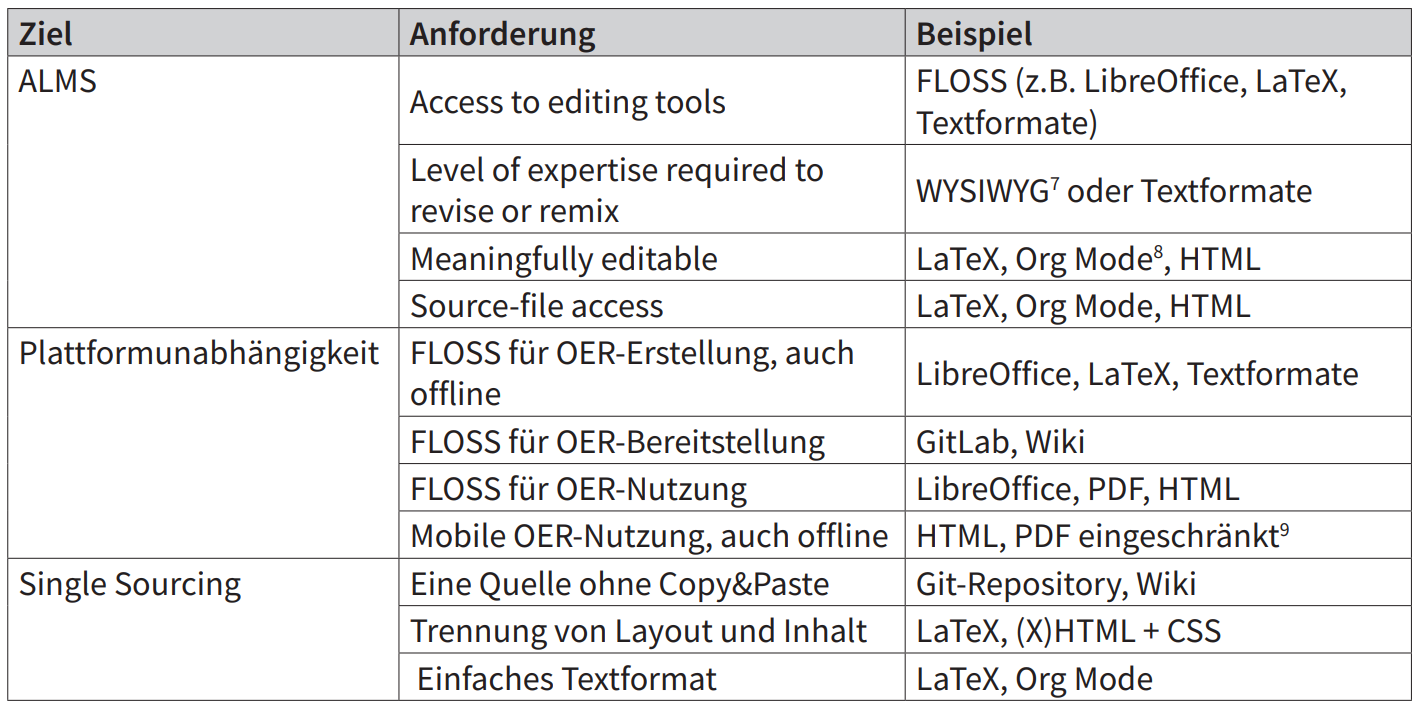
\includegraphics[width = 16cm]{alms_framework.png}
\caption{Anforderungen an OER-Software \cite{Lechtenborger.2019}}
\label{Anforderungen an OER-Software}

\end{center}
\end{figure}


Die zweite Anforderung des ALMS-Frameworks fordert eine möglichst geringe Expertise, die zur Nutzung der Software erforderlich ist. Hier sind Kundensegmente zu berücksichtigen, die eher eine geringere Affinität zu Computern aufweisen. Demnach ist die Benutzeroberfläche intuitiv zu gestalten und die Nutzung der Anwendung sollte auch ohne Programmierkenntnisse erfolgen können.

Die beiden letzten Kriterien des Frameworks sind eng miteinander verknüpft. Unter \glqq Meaningfully editable \grqq{} wird die Editierbarkeit der Materialien gefordert, während beim \glqq Source-file access \grqq{} dessen mögliche Verfügbarkeit verstanden wird. Sind die Quelldateien der Karteikarten nicht verfügbar, können die Karten folglich auch von keiner anderen Person bearbeitet werden. \\

Bei Plattformunabhängigkeit wird für die Erstellung, Bereitstellung und Nutzung der Materialien ebenfalls freie Software gefordert, die auch ohne eine Internetverbindung genutzt werden können und auch für mobile Endgeräte zur Verfügung steht. Eine weitere Anforderung, die zwar ebenfalls nicht mehr zum ALMS-Framework gehört, jedoch zur Weiterverarbeitung eine wichtige Rolle spielt ist das Prinzip \glqq Single-Sourcing \grqq{}. Die Trennung von Layout und Inhalt erleichtert die Weiterverarbeitung, auch innerhalb anderer Programme. Da Inhalt und Layout in separaten Dateien speicherbar ist, kann der Inhalt mit anderen Layout-Vorschriften versehen werden und sind nicht zuest zu separieren, welches redundante Arbeit eliminiert.  \\

Konsequenzen aus den Anforderungen von OER sind demnach die Veröffentlichung eines Quellcodes und die Entwicklung einer webbasierten Anwendung. Des Weiteren sind immer eine einfache Handhabung und kollaborative Funktionen, wie das Teilen und Weiterverarbeiten zu berücksichtigen. Die Anwendung soll jedem frei zugänglich zur Verfügung stehen und soll auch offline genutzt werden können. Durch die Einhaltung des Single-Sourcings könnten die Materialien auch in andere Anwendungen importiert werden, sofern Bedarf dazu besteht.

%\glqq committed and modified \grqq{}

\subsection{Methoden für ein effektives Lernen}
Damit das Gelernte nicht nur im Kurzzeitgedächtnis verbleibt und eine Reduzierung von Lernschleifen erreicht wird, werden Lernmethoden benötigt, die eine Speicherung in das Langzeitgedächtnis fördern. Aus vorhandener Literatur wurden drei Lernmethoden ausgewählt, die im Rahmen dieser Seminararbeit umgesetzt und im nachfolgenden Abschnitt erläutert werden.

\subsubsection{Leitner-Algorithmus}
Der heute wohl bekannteste Algorithmus zum Lernen von Karteikarten wurde von Sebastian Leitner im Jahr 1972 vorgestellt \cite{SebastianLeitner.1972}. Bei diesem Vorgehen werden die Karteikarten im Laufe einer Lernsession, entsprechend des Lernergebnisses von einer Phase in eine anderen Phase verschoben. Zu Beginn liegen alle neuen Karten in der niedrigsten Phase. Wird eine Karte richtig beantwortet, darf diese in die nächstgelegene Phase verlagert werden, ansonsten ist diese um eine Phase zurückzusetzen. Die jeweiligen Phasen unterliegen verschiedenen Zeitintervallen, meist in Einheiten von Tagen, die mit fortschreitenden Phasen stets zunehmen. Befinden sich Karten in einer der höchsten Phasen, sollte diese im Langzeitgedächtnis verankert sein. Im  Laufe der Zeit wurden weitere Versionen dieses Algorithmus entwickelt, bei denen beispielsweise die Karteikarte direkt in die erste Phase zurückgesetzt wird, nachdem diese falsch beantwortet wurde.

\subsubsection{Microlearning}
Eine weitere Lernmethode, die sich auch auf das Lernen von Karteikarten anwenden lässt, nennt sich Microlearning \cite{Hug.2005}. Hier wird das erfolgreiche Lernen durch temporär kurze Lerneinheiten unterstützt, die allerdings nur das wirklich relevante Wissen enthalten sollte. Nach dem Paper von Ilona Buchem und Henrike Hamelmann \cite{Buchem.2010} sollte eine Lerneinheit maximal 15 Minuten dauern. Da die Konzentrationsspanne eines Kindes zwischen 12 und 16 Jahren im Schnitt bei 30 Minuten und bei einem Erwachsenen im Schnitt bei 90 Minuten liegt, kann der Lernende innerhalb der Lerneinheit seine gesamte Konzentration einsetzen \cite{konzentrationsspanne}. Wissenseinheiten sollten in kleinen und unabhängigen Einheiten aufgeteilt werden, in denen jeweils nur ein Thema behandelt werden sollte. Nach Abschluss solch einer kurzen Lerneinheit bekommt der Lernende ein direktes Feedback, erhält somit eine positive Bestätigung und kann so seine Lernmotivation steigern.


\subsubsection{Spaced Learning}
Mit Wiederholungen (\glqq spaced repetition \grqq{}) der Lerneinheiten in bestimmten vorgeschriebenen Zeitintervallen, stellt das Spaced Learning eine Erweiterung zum Microlearning dar. Angelehnt wurde die Methode an die Vergessenskurve von Ebbinghaus aus 1880 und wurde erstmals theoretisch im Jahr 2005 von Douglas Fields eingeführt \cite{Fields.2005}. Zur Umsetzung des Spaced Learnings gibt es verschiedene Algorithmen, wie auf Basis von neuronalen Netzen \cite{BartoszDregerPiotrWozniak.1998} oder die Familie des SuperMemo-Algorithmus \cite{supermemo}. 


Die zugrunde liegende Theorie von Ebbinghaus sagt aus, dass nach 20 Minuten der Lernende nur noch 60{\%} des gelernten Wissens wiedergeben kann. Nach 60 Minuten liegt die Abrufmenge nur noch bei 45{\%}, nach 24 Stunden nur noch bei 34{\%} und nach 6 Tagen liegt die Abrufmenge lediglich bei 23{\%}. Von dem insgesamt gelernten Wissen bleiben lediglich nur 15{\%} dauerhaft gespeichert \cite{Liss.2020}. Um diesen Effekt zu vermeiden, sollten die kurzen, im besten Fall aufeinander aufbauenden Lerneinheiten in regelmäßigen Abständen wiederholt werden. \\

Eine Studie, die sich mit dem Vergleich zwischen Spaced-Learning und dem Massenlernen bei Honigbienen beschäftigt, fand heraus, beim Vergleich von Lernpausen von 30 Sekunden, 3 Minuten und 10 Minuten führten die Pausen von 10 Minuten zum besten Ergebnis \cite{Menzel.2001}. Diese konnten nach 30 Minuten zwar weniger Wissen abrufen, erreichten jedoch meist 100{\%} am dritten Kontrolltag, was auf eine Speicherung in das Langzeitgedächtnis hindeutet. \\

Diese Erkenntnisse, angewendet auf die Karteikarten-Anwendung führen, mit ausser Achtlassung bestehender Algorithmen, zum nachfolgenden Ergebnis. Eine Lerneinheit sollte aus einer Kategorie bestehen, kann aber auch bei Bedarf alle Karten in einer Kollektion berücksichtigen. Diese Lerneinheit hat eine maximale Dauer von 15 Minuten. Bei Beantwortung einer Frage wird ein Zeitstempel angelegt, der den Startzeitpunkt der nächsten Wiederholung festlegt. Nach Abschluss einer Lerneinheit kann, unabhängig von den Startzeiten der Karteikarten, die nächste Einheit frühstens nach 10 Minuten wieder gestartet werden. Ist diese Pause abgelaufen, sind die nächsten Karteikarten mit erreichen dessen Startzeit wieder aufrufbar.

%Eine andere Methode, wie sie in Anki eingesetzt wird ist die 

%Empfehlenswert sind 3 Einheiten zu einem Thema mit jeweils einer 10-minütigen Pause nach einer Einheit \cite{Kelley.2013b}. Diese Lernpausen können beispielsweise für unabhängige Zwischenspiele genutzt werden, um die Gedanken von dem Gelernten abzulenken. Ein weiterer Effekt dieser Lernmethode ist, wie auch beim Microlearning das regelmäßige und in kurzen Abständen auftretende Feedback, welches zu Erfolgsgefühlen führen und die Motivation steigern kann. 

%Weiterhin führen vielfältige Darstellungsformen, interaktive Elemente und ein Bezug in eigene Alltagserfahrungen und Alltagsgeschehen auch dazu, die Speicherung von Informationen in das Langzeitgedächtnis zu fördern. Im Rahmen der digitalen Verarbeitung können dazu vielfältige Methoden implementiert werden, die Abwechslung in die Einheiten bringen. Zum einen können mehrere Sinne angesprochen werden, wie mit einer Audioausgabe oder durch die Touchfunktion, wie auch mit verschiedenen Zwischenspielen. 



%http://super-memory.com/articles/theory.htm
%http://super-memory.com/english/algsm11.htm
%http://learnmem.cshlp.org/content/8/4/198.short


% Later research demonstrated two waves of transcription are required for LTM in honeybees: an early transcription wave (triggered during conditioning) and another starting several hours after learning (Lefer et al., 2012), as well as consolidation of LTM during sleep (Beyaert et al., 2012). 

\subsection{Berücksichtigung eigener Erfahrungen}
Nach mehrjähriger Erfahrung mit Karteikartenanwendungen kamen stets immer häufiger Änderungswünsche an der gerade genutzten Software auf. Diese Einblicke sind in dem Konzept der Anwendung berücksichtigt und werden nachfolgend kurz erläutert. \\

Eine Sortierung der Kurse nach definierten Prioritäten oder Fälligkeiten kann dabei helfen die Konzentration auf relevante, anstelle von nebensächlichen Kursen zu richten.

Zur Verwaltung von obsoleten Kursen könnte eine Funktion zur Deaktivierung implementiert werden. Wahlweise kann dies auch durch den Export von Kursen auf lokale Datenspeicher geschehen, um mögliche Serverkapazitäten einzusparen und die Daten zusätzlich sichern zu können. \\

Auch bei der Erstellung von Karteikarten gibt es einige Anforderungen, die aus meiner Sicht einen hohen Stellenwert haben. Zum einen sollte die Erstellung einfach und zügig erfolgen. Zum Anderen wäre eine Festlegung der Wichtigkeit von Karten sinnvoll oder die Festlegung von Prioritäten und Fälligkeitstermine für Kurse und Kategorien. 

Ein weiteres wichtiges Kriterium ist die Bearbeitungsmöglichkeit des Textes. Einige Anwendungen weisen hier schwere Mängel auf, die sich beispielsweise durch fehlende Hoch-, und Tiefstellungsmöglichkeiten bemerkbar machen. Da Karteikarten nicht mehr nur für das Lernen von Sprachen verwendet werden, sondern auch für mathematische oder chemische Kurse, ist eine Implementierung von Möglichkeiten zur Eingabe von Formeln notwendig. Viele Karteikarten-Anwendungen bieten nur die Möglichkeit diese Formeln als Bild zu speichern, was die Editierbarkeit jedoch einschränkt. Die Speicherung von Bildern ist eine weitere wichtige Anforderung, die hier erwähnt werden soll. Optimaler Weise wäre die Einbettung von Bildern im Textfluss, auch per einfacher copy {\&} paste Funktion, anstelle eines Filedialogs. \\

Zusätzlich zu den vorgestellten Lernalgorithmen könnten noch weitere Methoden implementiert werden, wie Abfragen ausgerichtet nach Fälligkeiten. Hier könnten die Karten und dessen Anzahl mit Hilfe von Prognosen festgelegt werden. Eine weitere Methode wäre die eigene Zusammenstellung von Karten innerhalb einer anderen Lernsession, um diese gezielt auswendig lernen zu können. Diese willkürlichen oder aufeinander abgestimmten Karten werden dann so oft wiederholt, bis alle Karten richtig beantwortet wurden. Die letzte hier gewünschte Lernmethode ist die Abfrage der zehn schwierigsten Karten, nach Fehlerquote festgelegt. Im Idealfall sollte der Nutzer in der Lage sein zwischen verschiedenen Lernmethoden wechseln zu können. 

Eine Funktion, die in jeder Lernmethode angewendet werden kann, ist die Auswahl der Lernrichtung für bestimmte Kategorien oder Kurse. Somit können beispielsweise Vokabeln in beiden Richtungen gelernt oder Antworten den entsprechenden Fragen zugeordnet werden. \\

Um eine visuelle Bestätigung und Belohnung zu erhalten sind grundlegende Statistiken erforderlich. Zu einer der grundlegenden Funktionen zählt die Auflistung der Karten in den jeweiligen Phasen, sowie der Aktivitätsverlauf für den Anreiz einer lückenlosen Lernaktivität. Nach einer Lernsession sollte eine Erfolgsquote visualisiert werden, um die Motivation zu steigern. Zusätzlich zu den Statistiken zum vergangenen und aktuellen Verhalten bzw. dem Lernstand sind Prognosen von fälligen Karten der nächsten Tage wünschenswert. \\

Für eine Individualisierung an eigene Bedürfnisse sind weitere verschiedenste Optionen notwendig. Beispielsweise mit inbegriffen ist die Festlegung der Anzahl von Karteikarten, die an einem Tag abgefragt werden, oder auch die Anzahl an neuen Karten, die täglich dazukommen können. Auch die Handhabung bei falsch beantworteter Fragen könnte hier definiert werden, wie die Zurückstellung in die Anfangsphase oder nur die Zurückstellung in die nächst zurückliegende Phase. Alternativ zu den Zeitintervallen der Phasen, könnte auch eine Wahrscheinlichkeit implementiert werden, die das Auftreten der Karten innerhalb einer Lernsession definiert. Zur Unterstützung der individuellen Lerngeschwindigkeit könnte auch eine Bestimmung der Anzahl von Phasen behilflich sein. 

% Sicherheit


\section{Evaluation vorhandener Software}
Zur Auswertung der Konkurrenzangebote wurden 5 gängige Karteikarten-Anwendungen identifiziert. Mit in der Evaluation inbegriffen ist die gewählte Implementierungsgrundlage, auf der die hier entwickelte Software aufgebaut wird. In der nachfolgenden Abbildung sind alle herausgearbeiteten Anforderungen und dessen Erfüllungsart in den jeweiligen Software-Produkten aufgelistet. Für jedes dieser Produkte werden anschließend noch nennenswerte Eigenschaften erläutert, die nicht in Abbildung 2 vorhanden sind.

\begin{figure}[htbp]
\begin{center}
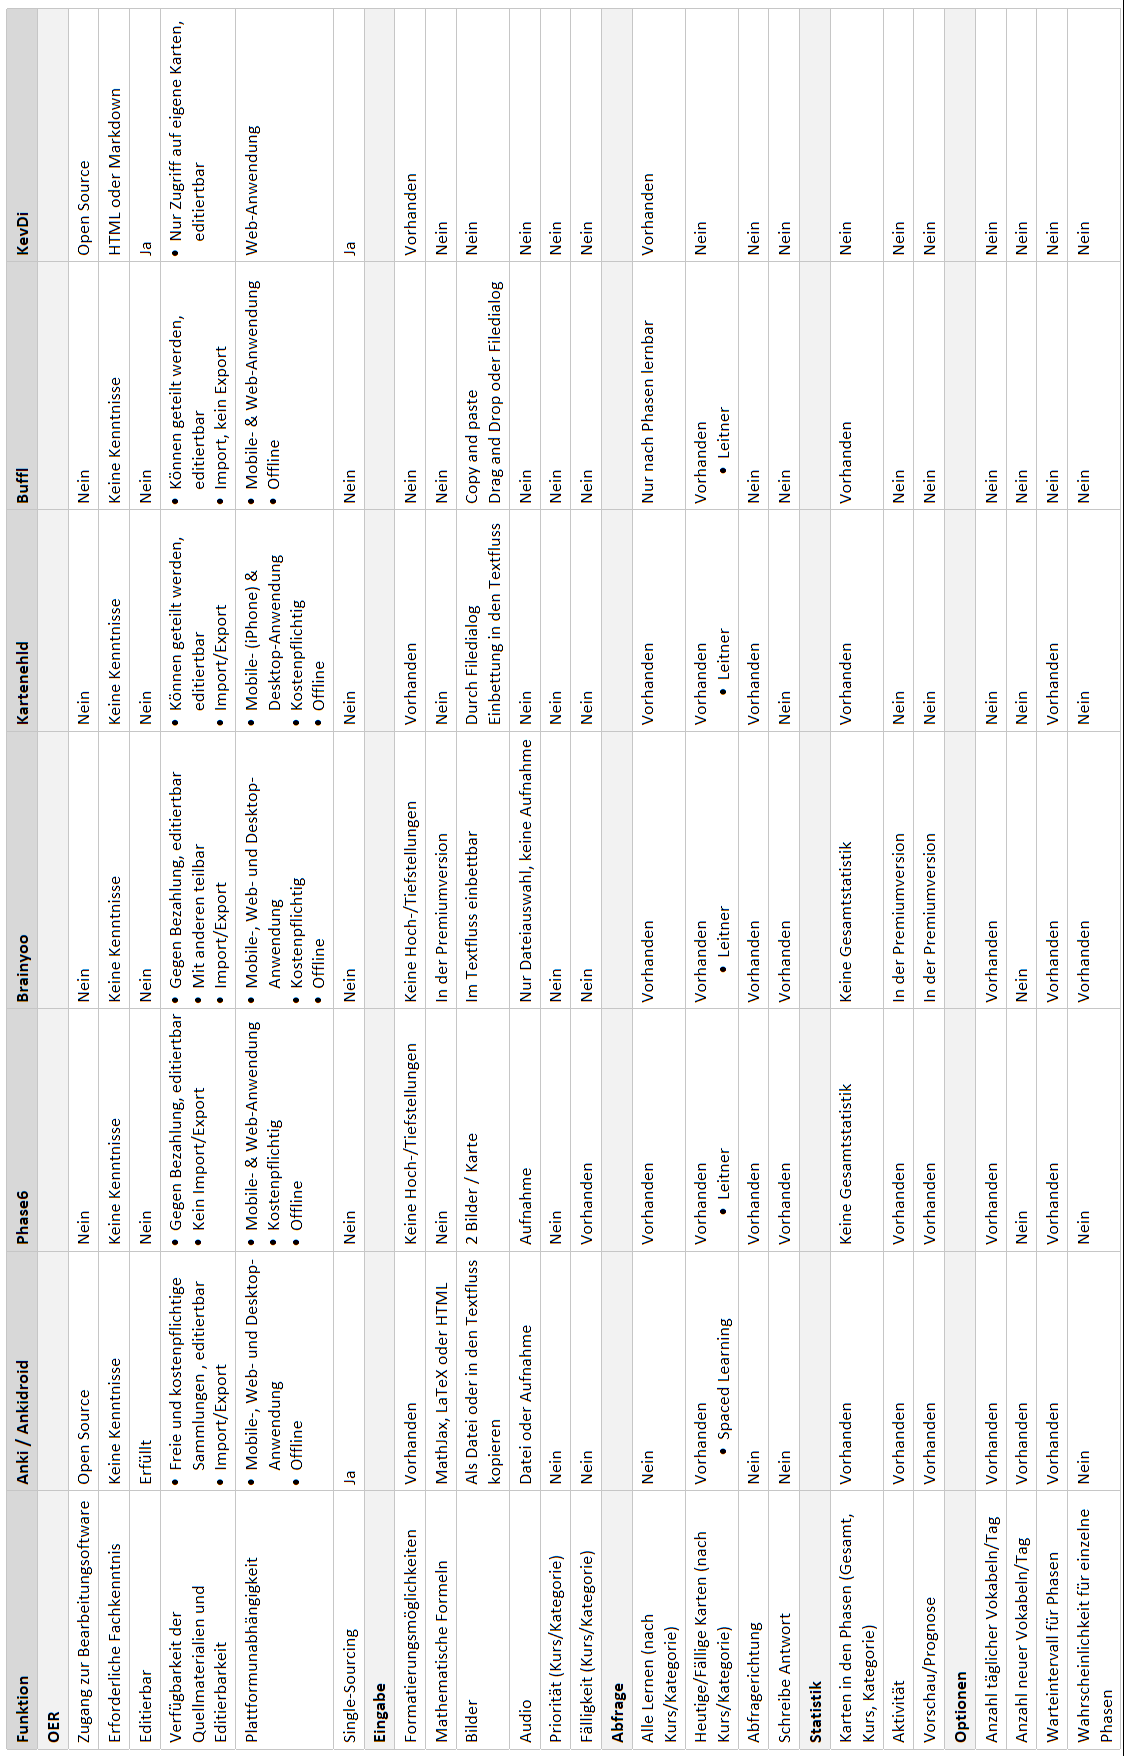
\includegraphics[width = 15cm, height=23cm]{evaluation.png}
\caption{Evaluation bekannter Karteikartenanwendungen}
\label{Evaluation bekannter Karteikartenanwendungen}

\end{center}
\end{figure}

\subsection{Anki und Ankidroid}
Die auf Open Source basierende Karteikarten-Applikation Anki \cite{ankiwebseite} \cite{ankidev} ist die funktionsstärkste Anwendung, die im Rahmen der Recherche gefunden wurde. Durch die Beliebtheit und der Möglichkeit einer gemeinschaftlichen Entwicklung arbeiten viele Entwickler an der fortlaufenden Verbesserung und Erweiterung. Erkenntlich wird dies beispielsweise bei der Eingabe von Karten. 

Eine Kartenseite kann in mehreren Sektionen aufgeteilt werden, die einen einheitlichen Aufbau vorschreiben. Im Beispiel von Vokabeln kann eine Karte in Wort, Bedeutung, Beispielsatz und einem Bild aufgeteilt werden. Weiterhin ist auch eine n-dimensionale Karte erstellbar, die nicht nur Frage und Antwort sondern beispielsweise auch eine Kartenseite mit einer Eselsbrücke enthält.  

Während der Eingabe können Bilder flexible und zügig per copy und paste in den Textverlauf eingefügt werden. Auch mathematische und chemische Formel können mit verschiedensten Methoden eingefügt werden. 

Im Bezug von Lernmethoden ist Anki eine von wenigen Karteikarten-Anwendungen, die Spaced Learning implementiert hat. Innerhalb der Statistik wird auch die Gedächtnisleistung nach Tageszeit berechnet. Eine hervorzuhebende Einstellungsmöglichkeit ist die Vermeidung von ähnlichen Karten, die sonst am selben Tag gelernt werden würden. Zur besseren Orientierung über die Qualität der vorgefertigten Karteikarten-Sammlungen hat Anki ein einfaches Votesystem auf der Webseite aufgeführt, die jeweils nur die Anzahl der guten oder schlechten Bewertungen angibt. Trotz der vielen Vorteile und erweiterten Funktionen lassen sich jedoch auch Kritikpunkte nennen. Zum einen ist das Design der Benutzeroberfläche auf der Desktop-Anwendung recht langweilig und trostlos gestaltet und folgt weniger modernen Designlayouts. Des Weiteren ist die Anwendung unübersichtlich gestaltet und mit den vielen Funktionen schon recht überladen. Die webbasierte Version von Anki beinhaltet noch nicht den vollen Funktionsumfang und ist noch in den Anfängen der Entwicklung.

\subsection{Phase6}
Um mit Phase6 \cite{phase6} sinnvoll Lernen zu können, benötigt der Benutzer mindestens die Silber-Premiumversion. Dies stellt auch einer der wesentlichen Kritik-Punkte dieser Applikation da. Ein weiterer Kritikpunkt ist, dass der Quellcode nicht öffentlich zur Verfügung steht und somit nicht zur gemeinschaftlichen Verbesserung geeignet ist. Ein zusätzliches Defizit bei Phase6 ist der fehlende Import/Export bzw. die Möglichkeit Kollektionen zu deaktivieren. Somit bleibt dem Nutzer nur die Möglichkeit diese vollständig zu löschen oder dauerhaft in der Anwendung zu belassen, was nach einiger Zeit jedoch ziemlich unübersichtlich werden kann. Nennenswert bei Phase6 ist jedoch die Option die Anzahl der Phasen individuell bestimmen zu können und die intuitive Benutzeroberfläche.


\subsection{BRAINYOO}
Wie auch bei Phase6 ist auch die Anwendung BRAINYOO \cite{brainyoo} für den Nutzer kostenpflichtig. Der Nutzer kann die Software jedoch für einen bestimmten Zeitraum testen. Für Unternehmen und Schulen besteht die Möglichkeit die Software auf Anfrage für den internen Einsatz auf eigene Server zu hosten und somit eine gemeinschaftliche Umgebung zum Lernen von Karteikarten für unterschiedlichste Zwecke zu bieten. Für jede Karteikarten-Kollektion können Lerngruppen erstellt werden, mit der gemeinsam an Kollektionen gearbeitet, bzw. gelernt werden kann. Jedoch ist BRAINYOO nicht für Linux-Distributionen geeignet, kann jedoch auf einem beliebigen Browser genutzt werden. Als Lernmethode bietet die Anwendung drei verschiedene Arten an. Zum einen einen Langzeitgedächtnismodus, der dem Leitner-System folgt. Ein weiterer Modus ist der Powermodus. Hier kann anstelle von Zeitintervallen eine Wahrscheinlichkeit für jede Phase angegeben werden. Der letzte Modus ist der Prüfungsmodus, in der alle Karten entweder sequentiell oder zufällig gelernt werden können. Für jede Karte kann zusätzlich zur Frage und Antwort eine Eselsbrücke angegeben werden, die beim Lernen helfen kann. 

\subsection{Kartenheld}
Die Anwendung Kartenheld \cite{kartenheld} ist eine ziemlich einfach gehaltene Software, die von Microsoft entwickelt wurde und dementsprechend auch dessen vertrautes Design folgt. Nach einer kostenlosen Testversion ist der Benutzer dazu verpflichtet sich eine Lizenz zu kaufen, was auf Grund der fehlenden Funktionen nicht empfehlenswert ist. Der Quellcode ist ebenfalls nicht für die Öffentlichkeit verfügbar. In Kartenheld ist es dem Benutzer nicht möglich Kategorien für einzelne Kurse zu erstellen, Statistiken einzusehen oder Einstellungen, abgesehen von den Zeitintervallen für einzelne Phasen zu treffen. Als einzige Statistik ist hier die Anzahl der Karteikarten in den einzelnen Phasen zu nennen. Positiv für Kartenheld ist jedoch die Möglichkeit Multiple Choice Aufgaben zu erstellen, die eine Abwechslung zum traditionellen Kartendesign darstellen. Auch die mögliche Abfrage nach schwierigen Karteikarten ist hier als nützliche Funktion zu nennen. Eine weitere Funktion ist die Auswahl der Phasen für eine Lernabfrage, auch wenn diese noch nicht für eine Abfrage fällig ist.

\subsection{Buffl}
Buffl \cite{buffl} ist eine funktional schlicht gehaltene Anwendung, die trotz dessen nicht intuitiv aufgebaut ist. Der Quellcode ist auch hier wieder nicht öffentlich verfügbar, doch für den Benutzer ist die Anwendung kostenlos. Die Kartenmodelle in Buffl sind mit verschiedenen Kartenmodellen eingeschränkt und es sind nur Kombinationen von Text, Listenpunkte und Bild möglich. Eine Kombination von allen drei Modellen ist hier nicht vorgesehen. Die Kurse können mit anderen per Link, E-Mail Adresse oder Benutzername geteilt werden. Auch ist ein Import aus dem eigenen System möglich, allerdings ist eine Exportfunktion bisher nicht vorhanden. 

\subsection{KevDi als Grundlage für die Entwicklung}
Die webbasierte Anwendung von KevDi \cite{kevdi}, die auf GitHub verfügbar ist, weist einen recht spärlichen Funktionsumfang auf. Die Benutzeroberfläche ist schlicht gehalten und macht einen benutzerfreundlichen Eindruck. Der Benutzer hat lediglich die Möglichkeit auf eigene Kurse und Karteikarten zuzugreifen. Für die Eingabe und die Formatierung von Texten für Karteikarten ist entweder die Sprache Markdown oder HTML notwendig, welches aber zur Wiederverwendung in anderen Programmen von Vorteil ist. In der untersuchten Version von KevDi ist es bisher nicht möglich Kurse zu bearbeiten oder weitere Kategorien für Kurse zu erstellen. Auch Bilder, mathematische Formeln oder das Abspielen von Audiodateien ist bisher nicht möglich. Als Lernmethode wurde weder das Leitner, noch das Spaced Learning implementiert. Hier hat der Nutzer nur die Wahl alle Karten eines Kurses zu durchlaufen bis alle Karten einmal beantwortet wurden. Im nächsten Durchlauf werden alle falsch beantworteten Fragen noch einmal wiederholt. Sind alle Fragen richtig beantwortet worden, müssen die Karten zurückgesetzt werden um eine erneute Abfrage starten zu können. In dieser Version sind bisher auch keine Einstellungsmöglichkeiten und Statistiken vorhanden. \\

Die Anwendung wurde trotz der mangelnden Funktionen als Entwicklungsgrundlage ausgewählt. Der Grund für diese Entscheidung ist unter anderem die schon vorhandene Benutzeroberfläche, die mit Hilfe der Python-Bibliothek Flask und den Designelementen von Bootstrap erstellt wurde. Zum anderen bot die Anwendung einen leichten Einstieg in den Quellcode und die Möglichkeit die Applikation von Grund auf aufzubauen, ohne die Funktionen zur Benutzerauthentifizierung zu implementieren. Auch die Anbindung an einen Web- und E-Mail Server sind schon vorhanden und so konnte sich auf die Implementierung der wesentlichen Funktionen konzentriert werden.





\section{Dokumentation der webbasierten Anwendung Kicards}
Auf Grundlage der vorher ermittelten Anforderungen und Funktionen aus den eigenen Erfahrungen und den evaluierten Softwareprodukten ist das Ziel dieser Seminararbeit eine webbasierte und effiziente Anwendung zu implementieren \cite{kicards}, die die Anforderungen von Open Educational Resources erfüllt. Nachfolgend werden zunächst alle benötigten Funktionen aufgelistet, die der Erfüllung der Anforderungen dienen. Anschließend werden zur Modellierungszwecke das Datenbankmodell, die Umsetzung der Lernmethoden und Funktionen zur kollaborativen Zusammenarbeit und Verwaltung von Karteikarten vorgestellt.


\subsection{Funktionsübersicht}
In der nachfolgenden Abbildung 3 wurden alle zu implementierenden Funktionen in must-, could-, und should-have Kategorien eingeteilt, um eine Priorisierung und einen Laufplan für die Entwicklung zu erhalten. Alle Funktionen innerhalb der must-have Kategorie sind unbedingt zu implementieren. In der should-have Kategorie sind alle Funktionen zu finden die eingearbeitet werden sollten und die Funktionen in der could-have Kategorie können bei Bedarf und Gelegenheit implementiert werden, sind allerdings nicht unbedingt erforderlich. \\

\begin{figure}[htbp]
\begin{center}
\includegraphics[width = 15cm, height=23cm]{must3.png}
\caption{Priorisierte Funktionen der Anwendung Kicards}
\label{Must-,Should-, Could-Have der Anwendung Kicards}

\end{center}
\end{figure}

Zunächst sind die Anforderungen im Sinne von OER zu finden, die alle in der must-have Kategorie eingeteilt wurden. Darunter fällt unter anderem die Forderung die benötigte Fachkenntnis zu reduzieren. Dies soll durch die Anzeige der wichtigsten Markdown-Sytnax, während der Erstellung und Bearbeitung von Karteikarten erreicht werden. Eine weitere Anforderung ist die Platformunabhängigkeit, die zunächst durch eine webbasierte Anwendung erfüllt wird. Die Freiheit der Bearbeitungssoftware und der Zugriff auf diese ist durch die Bereitstellung auf GitHub gewährleistet, in der auch Quellmaterialien zur Verfügung gestellt werden können. \\

Innerhalb der Rubrik Design ist ein notwendiges und damit unter must-have kategorisiertes Kriterium ein ansprechendes Design zu entwerfen, welches dem Nutzer zum Lernen motiviert. 
In der ersten Übersicht sollten abzuarbeitende Kurse ggfs. nach Prioritäten oder Fälligkeiten sortiert werden können. \\

Zur Erfüllung einer gemeinsamen Zusammenarbeit ist es unbedingt erforderlich Benutzerkonten zu erstellen. Einhergehend zum Benutzerkonto sollte der Nutzer dieses auch bearbeiten und löschen können. Weiterhin ist es erforderlich Kurse und dazugehörige Karteikarten zu erstellen. Kategorien und deren Unterkategorien sind zwar nicht notwendig, jedoch sollten diese dennoch implementiert werden, um eine bessere Organisation zu gewährleisten und den Empfehlungen des Spaced Learning, aufeinander aufbauende Inhalte zu lernen, nachzukommen. Für die Erfüllung der anderen vorgestellten Lernmethoden sollten Attribute wie Priorität, Fälligkeit von Kursen, wie auch Kategorien und Wichtigkeit der Karteikarten implementiert werden. Für eine eher allgemeinere Verwaltung der Kurse ist für die Applikation unbedingt eine Import- und Export-Funktion zu programmieren. Für die Unterstützung der Zusammenarbeit sollten private Kurse auch für die Öffentlichkeit bereitgestellt werden können. Damit die Karteikarten auch offline zur Verfügung stehen ist eine lokale Speicherung der Karten erforderlich. Allerdings ist hierfür eine mobile Anwendung oder Desktop Anwendung notwendig, die hier nicht mehr im Rahmen dieser Seminararbeit fällt. Um die Qualität der Karteikarten in Zusammenarbeit mit anderen zu steigern, müssen qualitativ minderwertigere Karten aussortiert werden. Hierfür ist ein Votesystem für Kurse und einzelne Karten notwendig, die allerdings auch hier unter der could-have Kategorie fallen.\\

Zur Erstellung von Karteikarten müssen entsprechende Kartendimensionen vorhanden sein. Notwendig ist die Kartendimension Frage und Antwort. N-dimensionale Kartenmodelle könnten noch implementiert werden, ist allerdings nicht erforderlich und fällt aus diesem Grund in die Kategorie could-have. Zur Formatierung der Texte könnten die Programmiersprachen Markdown und HTML genutzt werden. So sind die Formatierungen auch in andere Programme übertragbar und erfüllen somit auch die could-have Anforderung der Hoch- und Tiefstellung. Weitere Eingabemöglichkeiten die Implementiert werden sollten sind die mathematischen Formeln, Bilder und Audiodateien. Bilder per Copy und Paste in den Textverlauf einzufügen, fällt unter die Kategorie could-have, sowie ein Feld zur Darstellung der praktischen Anwendbarkeit in den eigenen Alltag. Dies ist auf das Konzept von Klaus Holzkamp zurückzuführen, der die Entstehung einer Handlungsproblematik als eine Motivation zum Erschließen von neuen Wissens darlegt. Problematisch ist die letzte Funktion im Zusammenhang mit geteilten Kursen. Hier müsste pro Benutzer ein individuelles Feld existieren. \\

In Bezug der Lernmethoden soll im Rahmen der Anwendungen das Leitner-System, sowie das Spaced Learning implementiert werden. Weitere Lernmethoden die unter der Kategorie should-have fallen sind das Lernen der schlechtesten Karteikarten, die Lernsession der selbst ausgewählten Karten innerhalb der intensiven Session, sowie das Lernen nach Fälligkeiten. Auch die Möglichkeit alle Karten oder die fälligen Karten nach Kurs oder Kategorie zu Lernen, sollten vorhanden sein. Eine weitere Funktion in der should-have Kategorie ist die Auswahl der Abfragerichtung. Eine Antwort zu schreiben oder Spiele zwischen den Lerneinheiten spielen zu können, zählen in die Kategorie could-have. \\

Statistiken können dem Benutzer dabei helfen seine Motivation zu steigern. Übersichten über Karten in den verschiedenen Phasen oder eine Übersicht über gelernten Karten nach einer Lernsession sind daher wichtig, um die Motivation beizubehalten. Neben diesen Statistiken können noch weitere, wie die über die Benutzeraktivität oder eine Prognose über in Zukunft anfallende Karten implementiert werden. Die in Anki eingebettete Statistik über die Gedächtnisleistung nach Tageszeit ist eine sehr nützliche Funktion, um sein Lernverhalten dementsprechend anzupassen, ist allerdings nicht notwendig, um dieses Projekt umzusetzen und fällt daher unter die could-have Kategorie.

Einstellungsmöglichkeiten, die unbedingt implementiert werden sollten, gibt es nicht. Lediglich als should-have können Optionen, wie die Anzahl der täglichen Vokabeln oder die Anzahl der neuen Vokabeln pro Tag bereitgestellt werden. Weitere Möglichkeiten betreffen die Ereignisse bei falscher Antwort oder das Warteintervall für einzelne Phasen. Zusätzliche hier aufgelistete Optionen, die allerdings in die could-have Kategorie fallen sind verwandte Karten nicht am selben Tag zu lernen oder eine Wahrscheinlichkeit für die einzelnen Phasen anzugeben. 




\subsection{Datenbankmodellierung}

Der nächste Schritt nach Festlegung der geforderten Funktionen besteht in der Modellierung der Datenbank. Hier wird im ersten Schritt das Datenbankmodell in Abbildung 4 skizziert und anschließend die Zusammenhänge und Abhängigkeiten erläutert.

\begin{figure}[htbp]
 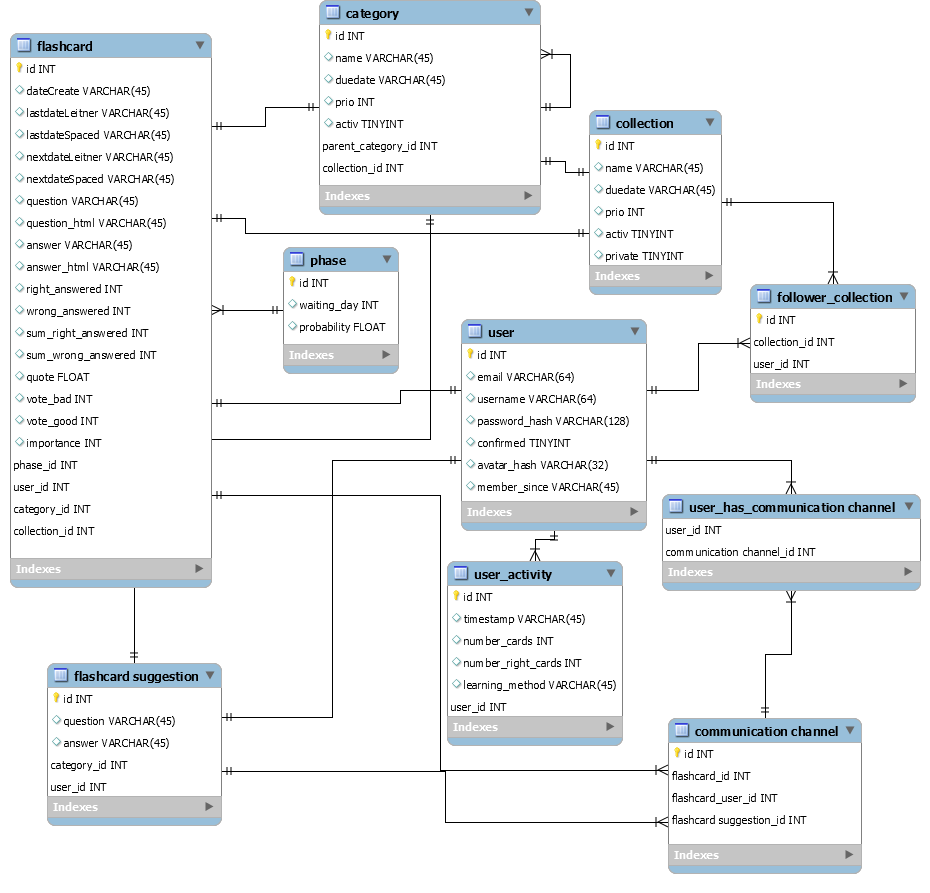
\includegraphics[width = 15cm]{databasemodel.png}
 \caption{Datenbankmodel von Kicards}
 \label{fig:datenbankmodel}
\end{figure}

% \glqq Text \grqq{}

Im Mittelpunkt des Datenbankmodells steht die Tabelle Karteikarte (\emph{flashcard}). Eine Karteikarte hat Attribute, wie die Phase (\emph{phasen{\_}id}), das Erstellungsdatum (\emph{dateBeginn}), jeweils ein Datum für die letzte Abfrage der Leitner-Methode (\emph{lastdateLeitner}) und ein Datum für den Spaced-Algorithmus (\emph{lastdateSpaced}), ebenso wie für die nächsten Abfragen (\emph{nextdateLeitner}, \emph{nextdateSpaced}). Für die Aufnahme der Frage und Antwort sind die Felder \emph{question} und \emph{answer} vorgesehen, die mit Hilfe einer Umwandlung in HTML auch die Felder \emph{question{\_}html} und \emph{answer{\_}html} belegen. Für die Ermittlung der Fehlerquote werden die Felder \emph{right{\_}answered} and \emph{wrong{\_}answered}, sowie die Summen \emph{sum{\_}right{\_}answered} and \emph{sum{\_}wrong{\_}answered} benötigt. Die Fehlerquote wird nach Aktualisierung in dem Feld \emph{quote} gespeichert. Um die Umsetzung des Votesystems für einzelne Karteikarten implementieren zu können, werden die Felder \emph{vote{\_}bad} und \emph{vote{\_}good} benötigt. Jede Karteikarte hat einen Ersteller, der in dem Attribut \emph{user{\_}id} gespeichert wird und eine Referenz zur Tabelle User enthält. Als letztes Attribut wird hier die Wichtigkeit (\emph{importance}) gespeichert. Jede Karteikarte gehört zu genau einer Kategorie und Kollektion, die jeweils durch die Felder \emph{collection{\_}id} und \emph{category{\_}id} modelliert wird.

In der Tabelle Kategorie (\emph{category}) befinden sich die Felder \emph{name} der den Namen der Kategorie enthält und das Feld \emph{duedate} für den Fälligkeitstermin. Zudem kann der Kategorie eine Priorität (\emph{prio}) zugeordnet werden. Um zu Bestimmen ob eine Kategorie gerade aktiv ist, d.h. zum Lernen bereitsteht, kann durch das Feld \emph{activ} ermittelt werden. Zu jeder Kategorie gehört eine Kollektion, die durch das Feld \emph{collection{\_}id} dargestellt wird. Jede Kategorie kann jeweils mehrere Unterkategorien enthalten, die durch das Feld \emph{parent{\_}category} dargestellt wird.

Die Tabelle der Kollektionen enthält ein Feld für den jeweiligen Namen (\emph{name}), ein Fälligkeitstermin (\emph{duedate}), eine Priorität (\emph{prio}) und auch ein Feld, um zu bestimmen, ob eine Kategorie aktiv ist oder deaktiviert wurde. Zusätzlich gibt es ein Feld, um zu Bestimmen ob eine Kategorie nur privat ist, oder für die Öffentlichkeit freigegeben wurde. 

Eine Kollektion kann von mehreren Benutzern verfolgt werden. Hierzu gibt es eine Tabelle \emph{follows{\_}collection}, die eine n:n-Beziehung zwischen Benutzer und Kollektionen darstellt. Zu diesem Zweck wird jeweils eine \emph{collection{\_}id} und eine \emph{user{\_}id} gespeichert. 

In der Tabelle Benutzer werden die E-Mail Adresse (\emph{email}), der Benutzername (\emph{username}), das Passwort in Form eines Passwort-Hashes (\emph{password{\_}hash}) und ein boolisches Feld gespeichert, in dem festgelegt wird, ob das Benutzerkonto bestätigt wurde. Zur Speicherung eines Benutzerfotos wird ein \emph{Avatar{\_}Hash} gespeichert. Als letztes Attribut wird hier das Erstellungsdatum des Benutzerkontos angegeben (\emph{member{\_}since}).

Die letzte Tabelle stellt die Aktivitäten des Benutzers dar. Diese wird hauptsächlich für die Ermittlung der Aktivitätsstatistiken verwendet. Hierzu wird der jeweilige Benutzer (\emph{user{\_}id}), ein Zeitstempel (\emph{timestamp}), die Anzahl der in einer Lernsession richtig beantworteten Karten, sowie die Gesamtzahl der Karten, die in dieser Session behandelt wurde. Als letztes Attribut wird noch die Lernmethode (\emph{learning{\_}method}) erfasst, um die Aktivität nach Methode filtern zu können.




\subsection{Funktionsdokumentation}
<<>noch in Arbeit>
In diesem Abschnitt der Funktionsdokumentation werden bedeutende Funktionen, die zur Erfüllung der herausgearbeiteten Anforderungen benötigt werden erläutert. Zunächst wird die Kartenabfrage behandelt mit Berücksichtigung der verschiedenen Lernmethoden. Anschließend werden Funktionen zur Verwaltung der Kollektionen und Karteikarten skizziert. Zum Schluss werden noch Funktionen zur kollaborativen Zusammenarbeit und Bearbeitung von Kollektionen und Karteikarten behandelt.

\subsubsection{Kartenabfragen}
<<>noch in Arbeit>
Zur Abfrage der Karteikarten im Sinne des Leitner-Systems wurden im Datenbankmodel die Phasen mit zugehörigen Wartezeiten oder auch wahlweise mit zugehörige Auswahlwahrscheinlichkeit skizziert. Während der Erstellung von Karten werden diese mit der ersten Phase 0 initiiert. Sobald die Leitner-Abfrage gestartet und eine Karte richtig beantwortet wurde, wird diese um eine Phase inkrementiert und das nächste Abfragedatum, entsprechend der aktuellen Phase um die jeweiligen Tage hoch gesetzt. Wurde diese jedoch falsch beantwortet, wird die Karte um eine Phase zurückgesetzt und das nächste Abfragedatum bleibt unberührt. Gleichzeitig, egal wie die Karte beantwortet wurde wird das letzte Abfragedatum \emph{last{\_}date{\_}leitner} auf den aktuellen Zeitpunkt gesetzt. \\

Beim Spaced-Learning Algorithmus werden die Fragen nicht mit Richtig oder Falsch beantwortet, sondern wird in die jeweilige Qualität leicht, mittel und schwer eingeordnet. Karten die in der Kategorie leicht zugeordnet wurden, werden innerhalb der nächsten xx Tage nochmal abgefragt. Karten in der Kategorie mittel werden in den nächsten 60 Minuten nochmals abgefragt und die Karten in der Kategorie schwer in den nächsten 10 Minuten. Hierzu wird jeweils dementsprechend das nächste Abfragedatum verändert. \\

Im Falle der Lernmethode \glqq{}schlechtesten Karten \glqq{} werden aus der ausgewählten Kollektion alle Karten ermittelt. Von diesen ermittelten Karten werden jeweils die 10 schlechtesten identifiziert und zur Lernsession hinzugefügt. Diese werden solange wiederholt bis alle Karten richtig beantwortet wurden. \\

Die Lernmethode nach Fälligkeit ist aufwändiger zu Implementieren. Hierzu ist eine Prognose erforderlich, die ermittelt wie viele Karten durchschnittlich im Laufe eines Tages gelernt werden müssen um den Termin einzuhalten. Hier können zudem noch einige Tage als Puffer berücksichtigt werden, die vom Fälligkeitstermin abgezogen werden. Innerhalb eines Lerntages wird anschließend die Anzahl der noch zu lernenden Karten angezeigt, um das Ziel zu erfüllen. \\

Während einer Abfrage oder der Erstellung von Karten kann jeweils die Wichtigkeit von 0 (nicht wichtig) bis 5 (sehr wichtig) angegeben werden. Beim Start der Abfrage kann der Nutzer festlegen, welche Wichtigkeit bzw. Wichtigkeiten er lernen möchte. Hierzu werden aus der ausgewählten Kollektion alle zugehörigen Karten abgefragt und dem Benutzer in der Lernsession angezeigt. \\

Die Kartenauswahl für das intensive Lernen kann in jeder Abfrage mit dem Button \glqq für später merken\grqq{}
 ausgewählt werden. Kehrt der Nutzer zur Übersicht der Kollektion zurück, kann dieser die intensive Session mit den ausgewählten Karten starten. Nach einem Durchlauf der Lernsession wird diese nochmals neu gestartet für den Fall falls mindestens eine Karte falsch beantwortet wurde. Wurden im Gegensatz dazu alle Karten richtig beantwortet wird die Lernsession beendet.

\subsubsection{Verwaltung von Karteikarten}
<<>noch in Arbeit>





\subsubsection{Kollaboratives Lernen und Bearbeiten}
<<>noch in Arbeit>
Um das kollaborative Arbeiten zu Unterstützen sind Funktionen, wie das Importieren der Karten in öffentliche Kollektionen und ein Votesystem für die Qualität der Karten erforderlich. 

Um eine öffentliche Kollektion zu erstellen, muss eine private Kollektion für die Öffentlichkeit freigegeben werden. Dies geschieht durch das Bestätigen eines Buttons. Mit der Freigabe ist es anderen Benutzern möglich dieser Kollektion zu folgen und auch Karteikarten in diese zu importieren. 

Zu diesem Zweck kann der Benutzer aus der Kartenübersicht verschiedene Karteikarten auswählen und mit Auswahl der öffentlichen Kollektion, die Karten hinzufügen. 

Für eine Gewährleistung der Qualität ist ein Votesystem innerhalb der Kollektion erforderlich. Sobald die schlechten Votes der Anzahl der Follower um 80{\%} übersteigt, wird die Karte aus der Kollektion gelöscht. Eine Problematik die hier berücksichtigt werden muss, ist die Löschung der Follower aus der entsprechenden Tabelle, wenn diese eine Inaktivität von beispielsweise 90 Tagen aufweisen. 


\section{Ausblick}
<<>noch in Arbeit>
Im Rahmen dieser Seminararbeit konnte der volle Funktionsumfang der webbasierten Anwendung noch nicht implementiert werden. Im Abschnitt der Weiterentwicklung werden bereits implementierte Funktionen in Abbildung 5 skizziert und der weitere Verlauf der Weiterentwicklung, sowie Einsatzmöglichkeiten dargestellt. Zusätzlich wird im Kapitel Einsatzmöglichkeiten die zukünftige Anwendung und mögliche Kundensegmente der Software identifiziert.

\subsection{Weiterentwicklung}
<<>noch in Arbeit>
Zur besseren Übersicht der bereits implementierten Funktionen wird auf die Tabelle der must-, should- und could-have Anforderungen zurückgegriffen, die in der nachfolgenden Abbildung 5 dargestellt wird.




\subsection{Einsatzmöglichkeiten}
<<>noch in Arbeit>
Es gibt vielfältige Einsatzmöglichkeiten für die hier entwickelte Karteikarten Anwendung. Hauptsächlich kann diese für jeden auf einem öffentlichen Webserver zur Verfügung gestellt werden. Für interne Einsätze dieser Software ist es möglich diese auf eigene Server zu hosten. So können beispielsweise Universitäten, Schulen und Unternehmen ihren Studenten, Schülern und Mitarbeitern die Möglichkeit bieten ihr Wissen zu bestimmten Thematiken zu festigen. Für die Institute hat dies den Vorteil von gebildeteren und besser geschulten Personal. Für Schulen und Universitäten kann dies ein höheres Ansehen durch fortschrittlichere Lernumgebungen ermöglichen. Auch weitere Einsatzmöglichkeiten zu den traditionellen sind möglich. So können beispielsweise auch Nachhilfelehrer oder Plattformen, wie coursera.de diese Software für Ihre Zwecke nutzen. Da der Quellcode für jeden öffentlich zur Verfügung steht, ist der Einsatz auch mit keinerlei Kosten verbunden und dient hauptsächlich zur Förderung der Bildung und somit zur Festigung von Wissen in das Langzeitgedächtnis.


% The following is for the Emacs users out there... :-)
%%% Local Variables:
%%% mode: latex
%%% TeX-master: "guide2seminars"
%%% eval: (ispell-change-dictionary "en")
%%% End:


  % Include (1) literature and (2) web references in separate BibTeX files
  \dbisbibliography{LiteratureSample}{WebReferencesSample}

%  \section*{\appendixname}
%  \appendix
%  \section{Test}
%  No real text here, just a test appendix.  For bachelor and master
%  theses, you should use chapters in the appendix, not sections.

  % Make sure that final declarations start on separate page.
  \newpage
\end{document}

% The following is for the Emacs users out there... :-)
%%% Local Variables:
%%% mode: latex
%%% TeX-master: t
%%% End:
